This chapter describes the search for a neutral MSSM Higgs boson decaying to a pair of $\tau$. The studied final state is defined by the presence of a pair of reconstructed hadronic $\tau$ decays, and this channel is thus named \tauh\tauh. The Standard Model Higgs boson decay into a pair of $\tau$ leptons has been discovered by both the CMS and ATLAS collaborations \cite{ATLASHtt,CMSHtt}. In the context of the MSSM, three neutral Higgs bosons are predicted: the CP-even states h and H and the CP-odd state A, which may all decay to $\tau$ pairs. A model-independant search for a single Higgs boson, denoted $\phi$, is performed in a mass range of $90$ to $3200\,\mathrm{GeV}$. The analysis is sensitive to production via gluon-gluon fusion and production in association with b-quarks. The cross section of the latter increases for larger values of $\mathrm{tan}\beta$ due to the enhanced down-type fermion Yukawa couplings.  The search is also performed in the $m_A - \mathrm{tan}\beta$ parameter space of the $m_{h}^{max}$ scenario \cite{Carena2003} for the same mass range.

Similar searches for MSSM neutral Higgs bosons have previously been performed by the collaborations at LEP \cite{Schael2006}, the Tevatron \cite{Benjamin:2010xb}, and at LHC by the CMS and ATLAS collaborations \cite{Aaboud2018,Sirunyan2018} with no excess observed above the background expectation. 

The results presented here follow those published by CMS in 2018 using 2016 data, but makes use of the new 2017 data for the first time while being restricted to the \tauh\tauh channel. The 2017 data corresponds to an integrated luminosity of 41.5 $\mathrm{fb^{-1}}$. Event categorisation is used to enhance sensitivity to particular production modes. The production of neutrinos in the $\tau$ decays makes it difficult to reconstruct the invariant mass of the candidate Higgs boson. Statistical inference is therefore performed on the distribution of the \mttot variable, designed to account for \MET in the mass estimation, and therefore to improve signal to background separation.

Section \ref{sec:analysis_samples} outlines the datasets of recorded collisions, defined by which trigger these collisions fired, and the simulation used to estimate the contribution of some of the background processes. The event selection, which is done in a framework partially developed for this purpose is then detailed in section \ref{sec:analysis_eventsel}. The estimation of the contribution of each background processes, using data-driven methods where possible, is detailed in section \ref{sec:analysis_background_methods} and followed by a summary of the experimental and theoretical uncertainties affecting the signal and background estimations in section \ref{sec:analysis_systematics}. The statistical procedure used to quantify the presence of signal in the data is given in section \ref{sec:analysis_statistical_interpretation} and is followed by the results of the search in section \ref{sec:analysis_results}.

\section{Data samples and simulation}
\label{sec:analysis_samples}

\subsection{Trigger}
Collision datasets are defined by the trigger pattern that fired their recording. At both the level one (L1) trigger and the high level trigger (HLT), the trigger patterns are defined by requirements of reconstructed objects. The definition of these trigger objects vary from level to level, as the complexity of the reconstruction techniques increase at each level, as the rate at which events must be treated lowers. Therefore, the object properties determined in the trigger reconstruction, such as \pt and isolation, are only approximate to those in the full reconstruction.

Events are first selected at the L1 trigger level by an algorithm requiring either one L1 \tauh of $\pt > 70\,\mathrm{GeV}$ and $|\eta| < 2.1$, or two L1 \tauh of $\pt > 28\,\mathrm{GeV}$ and $|\eta| < 2.1$. At the HLT level, the di-\tauh triggers require two HLT \tauh objects to be isolated, identified, to not overlap, and to each have $\pt > 35\,\mathrm{GeV}$ and $|\eta| < 2.1$. In the analysis, the full reconstruction \tauh candidates are required to have $\pt > 40\,\mathrm{GeV}$. Such requirements are referred to as offline selections. Since the reconstruction at trigger level is not as complete as the full reconstruction, events that pass the offline selections can be rejected at the HLT level. The trigger efficiency with respect to the offline selections typically plateaus at $85\%$ for large \tauh \pt \cite{Sirunyan_2018}. At the \pt threshold applied in the analysis, it is around $60\%$. 

\subsection{Trigger optimisation}

In order to maximize the trigger efficiency for our analysis, asymmetric \pt thresholds have been considered at the HLT level. The main goal of this study was finding a set of \pt thresholds that would improve efficiency without increasing the trigger rate. 
In order to estimate the efficiency gain, a new trigger pattern similar to the classical double \tauh trigger but without any \pt requirements was implemented. It was then applied to simulated datasets of $H\rightarrow \tau\tau$ and DY $Z\rightarrow\tau\tau$ events. The \pt requirements on the trigger-level objects were then applied after the full reconstruction on the HLT level \tauh trigger objects to simulate the use of new \pt thresholds, and the efficiency was calculated as
\begin{equation}
    \epsilon = \frac{n_{\mathrm{trigger}}}{n_{\mathrm{selection}}} \mend
\end{equation}
In this expression, $n_{\mathrm{trigger}}$ is the number of these events that pass the trigger \pt requirements. The number $n_{selection}$ is the number of events that pass the analysis selection, which are that two offline reconstructed \tauh are found in the event, and that these \tauh pass the tight WP of the BDT-based identification criterion defined in chapter \ref{sec:RECNNchapter} and the kinematic cuts of $\pt > 40\,\mathrm{GeV}$ and $|\eta| < 2.1$ . This efficiency is then computed for different values of \pt requirements for each of the two \tauh trigger objects.

To estimate the firing rate in real collisions, the trigger pattern without \pt requirement was then applied to randomly selected collision events, to avoid introducing bias from the use of a trigger.  The rate were then computed from the random selection rate as
\begin{equation}
    f = \frac{n_{\mathrm{pass}}}{n_{\mathrm{total}}} \times f_{\mathrm{unbiased}} \mend
\end{equation}
In this expression, $n_{pass}$ is the number of events that pass the trigger threshold, $n_{total}$ is the total number of events of the unbiased sample, and $\mathrm{f}_{\mathrm{unbiased}}$ is the rate of random selection used to produce the unbiased sample. 

\begin{figure}
    \centering
    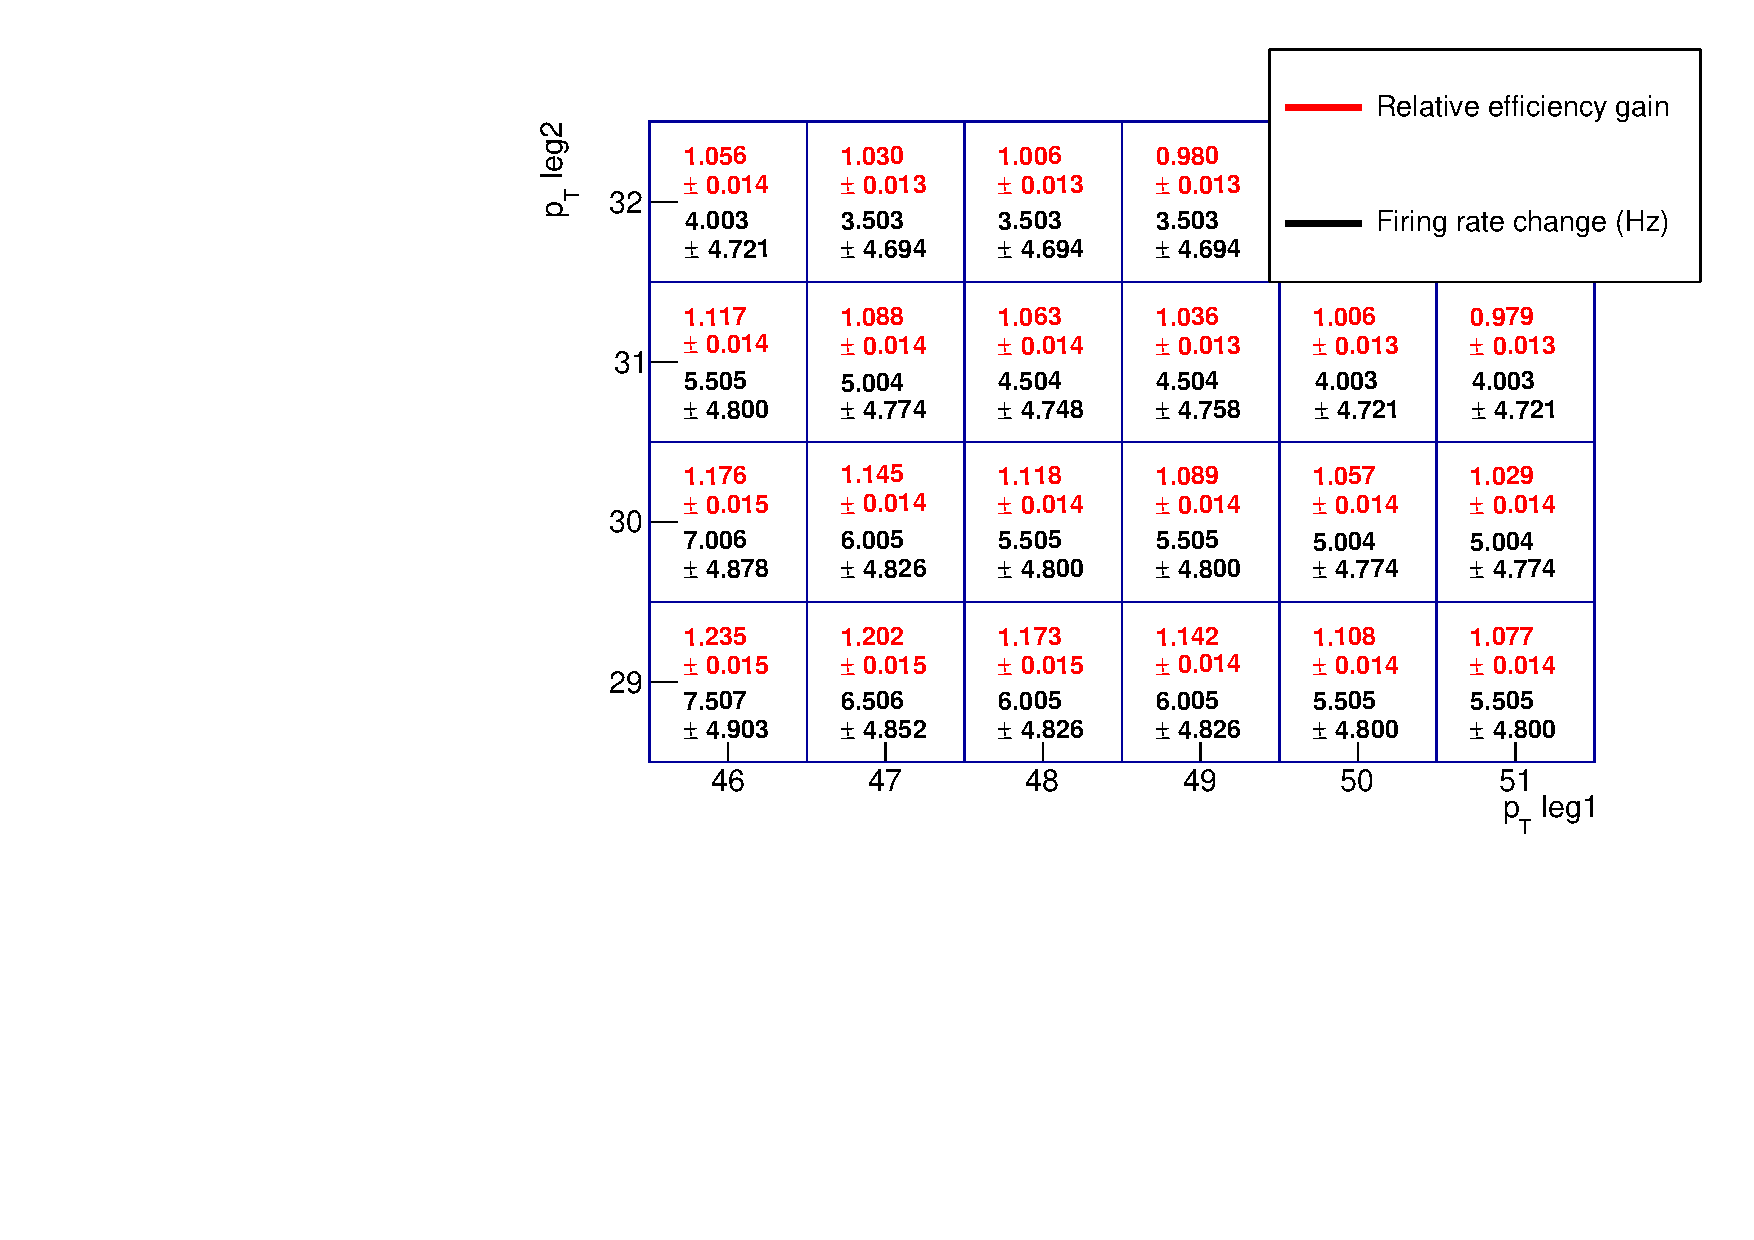
\includegraphics[width=0.8\textwidth]{Images/asym_results.pdf}
    \caption{Values of the relative efficiency gain and the firing rate increase for different values of \pt thresholds. The displayed uncertainties are only statistical. The complete studied range was $35$ to $60\,\mathrm{GeV}$ for the leading HLT \tauh object and $20$ to $40\,\mathrm{GeV}$ for the sub-leading, but only the region that was found to be most interesting in terms of efficiency gain and rate increase is diplayed here.}
    \label{fig:asym}
\end{figure}

Some of the results are shown in Figure \ref{fig:asym}. The statistical uncertainties on the measured rates are very large due to the very low number of events passing the offline selection in the randomly selected datasets. This study showed a gain of up to $6\%$ in efficiency through the use of asymmetric trigger thresholds, while the rate was kept unchanged within the statistical uncertainties. But before more unbiased datasets were used to lower the uncertainties, a $Z\rightarrow \tau\tau$ polarisation analysis showed the use of such a trigger pattern could reduce their acceptance of about $20\%$. The use of asymmetric \tauh trigger \pt threshold was therefore not implemented by the CMS collaboration.

\subsection{Simulation}
In the analysis, several Monte Carlo (MC) generators are employed to produce simulated samples of signal and background events. The MADGRAPH \cite{Alwall2011} matrix element generator is used for Z+jets, W+jets, $\mathrm{t\Bar{t}}$+jets and diboson production. The POWHEG \cite{Alioli2010} generator is used for single top-quark production. The SM gluon-gluon fusion and VBF production modes of the Higgs boson, treated as a background in this analysis, are also simulated with POWHEG at NLO precision. Both ggH and bbH MSSM signal production modes are provided by PYTHIA \cite{SJOSTRAND2008852}. All samples utilise PYTHIA for parton showering and hadronisation, and TAUOLA \cite{JADACH1991275} for tau decays.


\section{Analysis sequence}
\label{sec:analysis_eventsel}

This section describes the event-based analysis sequence. The goal of this sequence are applying an event selection, applying corrections to the reconstructed physics objects and to derive quantities such as weights and physical variables like \mttot, the final discriminating variable. The interpretation will be done from the distribution of this variable, defined as 
\begin{equation}
    \mttot = \sqrt{m_{\mathrm{T}}^2(\tauh^{(1)},\MET) + m_{\mathrm{T}}^2(\tauh^{(2)},\MET) + m_{\mathrm{T}}^2(\tauh^{(1)},\tauh^{(2)})}
\end{equation}
where
\begin{equation}
    m_{\mathrm{T}} (x,y) = \sqrt{2\times \pt^x \times \pt^y \times (1-\mathrm{cos}(\Delta \phi_{x,y}))} \mend
\end{equation}
In these expressions, $\tauh^{(1)}$ and $\tauh^{(2)}$ are the selected pair of offline \tauh. The \tauh pair selection process is detailed later in this section. The variables $\pt^x$ and $\pt^y$ are the \pt of objects $x$ and $y$ respectively, and $\Delta \phi_{x,y}$ is the angle between the projection of the 4-momentum of objects $x$ and $y$ in the transverse plane. 

To maximize the sensitivity, the \mttot distributions are derived in two categories. The categories are designed around the b-associated production of Higgs bosons, which is favored at high $\mathrm{tan}\,\beta$ values. The events are then categorised from the presence of a b-tagged jet, leading to two distinct categories, one called the b-tag category where at least one b-tagged jet is found in the events, and the other called the no b-tag category defined by the absence of any b-tagged jet in the events. 

% First, we will provide an overview of the framework used to process data and simulation events in this analysis, called heppy. This will be followed by a description of the analysis sequence.

To create the distributions, data and simulation events are first processed using a framework called heppy. Heppy is a python event processing framework for high energy physics based on ROOT. While it can take different ROOT-based type of inputs, the inputs used in this analysis follow the MINIAOD format of the CMS collaboration. This format was designed to hold the event-based information needed by most analyses. Therefore, the input files hold a lot of information, i.e. the lists of reconstructed physics objects, making it quite important in size. Events are first selected along the criteria defined in this section, while also trimming the information that is not useful to the analysis, leading to a new lightweight format. 

Heppy is a modular framework, which means that all the processing is done in a feed-forward workflow with each step being encoded into a module called analyzer. Physics objects retrieved from the ROOT files are wrapped in python classes, allowing definition of useful methods. Most analyzers of this workflow manipulate the physics objects to either create new useful variables, create lists of objects passing a criterion or reject events based on specific criteria. New analyzers have been created in order to provide as much modularity and clarity as possible so that other channels and any equivalent stages of future analyses will be able to easily and promptly be implemented.


\begin{figure}
    \centering
    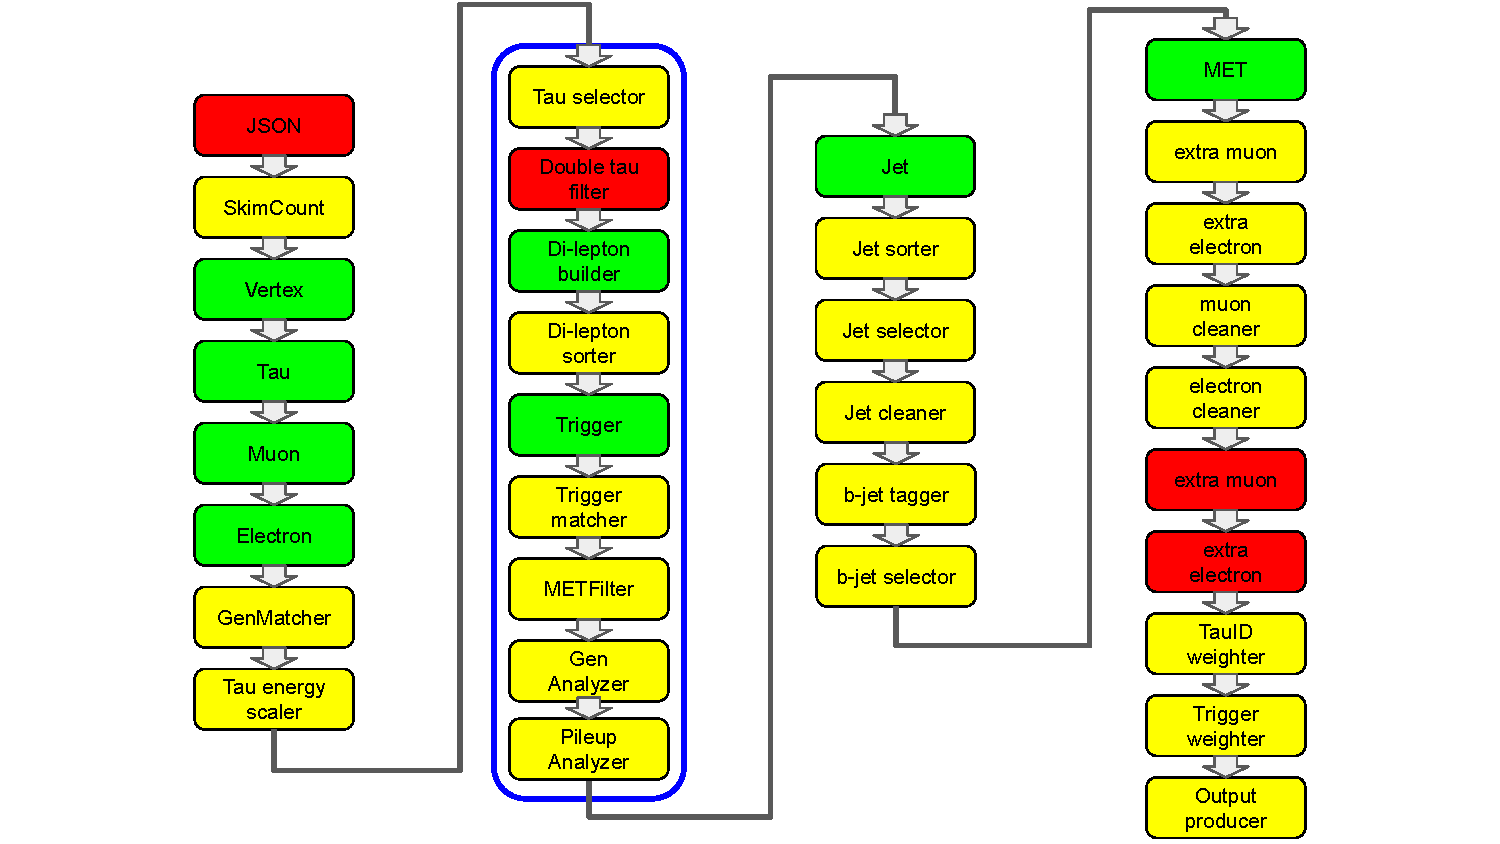
\includegraphics[width=\textwidth]{Images/HEPPY_diagram.pdf}
    \caption{Diagram of the selection flow implemented in heppy. Every box represents a module, called analyzer. Green analyzers create collections in the event instance by wrapping objects from the input in dedicated python classes. Yellow analyzers modify or compute a variable of the event. Red analyzers reject events that do not match given selection criteria. Finally, the blue highlighted section is the only part of the sequence that is specific to the $\tauh\tauh$ channel. The rest of the sequence is used in other channels, like the semileptonic channels $e\tauh$ and $\mu\tauh$, and has been successfully tested.}
    \label{fig:HEPPY}
\end{figure}

The following paragraphs are focused on the description of the sequence for the \tauh\tauh channel. This sequence is applied to both simulation and data, some analyzer being specific to either simulation or data. A diagram of the workflow is shown in figure \ref{fig:HEPPY}. In the order of use in the analysis flow, the role of the analyzers are the following:
\begin{itemize}
    \item JSON: Only active when running on real data. Rejects the events that have not been validated by the CMS collaboration.
    \item SkimCount: Only active when running on simulation. Counts the number of generated events before selection. This is used later to renormalize the number of generated events to match the data integrated luminosity.
    \item Vertex: creates a collection of the vertices that passed quality criteria \cite{tracker}. These quality criteria are applied in order to select genuine pp interactions and reject beam-induced backgrounds. If several of such vertices are found, the vertex with the highest scalar sum of associated track \pt is assumed to be the primary vertex.
    \item Tau/Muon/Electron: creates collections of the respective objects, and adds useful methods and attributes to these objects.
    \item Gen matcher: Only active when running on simulation. Matches reconstructed \tauh with closest generator-level particles, and classify them following the scheme described in table \ref{tab:mc_matching}.
    \item Tau energy scaler: only active when running on simulation, scales the energy of \tauh, depending on their gen level match. Stores each changes for later propagation to the \MET.
    \item Tau selector: first analyzer of the channel-specific sequence. Selects \tauh which have:
    \begin{itemize}
    \item $\pt > 40\,\mathrm{GeV}$ and $|\eta| < 2.1$;
    \item passed the decay-mode finding discriminator detailed in section \ref{sec:std_tau_id};
    \item $d_z < 0.2\,\mathrm{cm}$, where $d_z$ is the longitudinal distance between the ppoint of closest approach of the leading charged track and the selected primary vertex;
    \item passed the very loose working point of the anti-electron discriminator and the loose working point of the anti-muon discriminator.
    \item passed the loosest WP of \tauh BDT-based identification criterion. While the signal region is defined by both selected \tauh passing the tight WP, events with \tauh passing the loosest and not the tight WP identification criterion are used for the fake factor method as will be described in section \ref{sec:ff}, and should therefore also be selected.
    \end{itemize}
    \item Double tau filter: Rejects the event if less than two \tauh fulfilling the requirements of the Tau selector have been found.
    \item Di-lepton builder: creates all possible combinations of two \tauh that have passed the selections, provided the \tauh:
    \begin{itemize}
    \item are separated by $\Delta R > 0.5$.
    \item have opposite-sign electric charges.
    \end{itemize}
    \item Di-lepton sorter: After these requirements, several pairs of \tauh candidates can remain. In this case, the pair with the \tauh of highest \pt, called leading \tauh, is chosen. If two pairs have the same \pt for their leading \tauh, the pair with the most-isolated leading \tauh is chosen. In case of more than one pair with the same leading \tauh \pt and isolation, the next tested criterion is the \pt of the other \tauh and the last criterion is the isolation of this other \tauh.
    \item Trigger: Retrieves the trigger information
    \item Trigger matcher: Checks if the selected \tauh pair matches with any of the L1 trigger patterns, and any of the HLT trigger patterns.
    \item MET Filter: Retrieves several flags that are provided by the CMS collaboration to reject events in order to mitigate several \MET reconstruction issues.
    \item Gen analyzer: Only active when running on simulation. Retrieves generator-level information in order to compute several weights, i.e the top quark and Drell-Yan \pt reweighting that are detailed in the next section.
    \item Pileup analyzer: Only active when running on simulation, retrieves pileup information and computes pileup weights, as detailed in the next section.
    \item Jet: Creates collection of jets, and adds useful methods and attributes. Also applies the jet energy corrections as detailed in next section, while also storing the information for propagation to the \MET.
    \item Jet sorter: Sorts the jet collection by \pt.
    \item Jet selector: Jets are required to have $\pt > 30\,\mathrm{GeV}$ and $|\eta| < 4.7$, and to pass identification criteria to reject fake jets originating from detector noise, and pileup jets.
    \item Jet cleaner: Discards jets overlapping with one of the two selected leptons, i.e. the distance between jets and any lepton must be $\Delta R > 0.5$.
    \item b-jet tagger: Applies a tag to each jet that defines if it is considered as a jet originating from a b-quark (b-tagged). The medium WP of the deepCSV method \cite{Sirunyan_2018} is used. Also applies b-tagging corrections as detailed in the next section.
    \item b-jet selector: Creates a b-tagged jet collection from all jets passing the b-tagging requirements defined in the b-jet tagger, and of $|\eta|<2.5$.
    \item MET: Retrieves \MET of the event. Applies all needed corrections detailed in the next section and adjust the \MET to compensate for all corrections applied to other physics objects.
    \item extra muon (electron) cleaners: Rejects events if any muon (electron) passes a set of quality criteria.
    \item TauID/trigger weighters: compute and apply the respective correction weights detailed in the next section.
    \item Output producer: Gathers all desired information and stores it in a flexible ROOT format allowing production of the distributions for statistical inference.
\end{itemize}

The output of this stage is used to perform a synchronisation with other CMS institutes working on the same analysis. For example a prototype of this sequence was used to synchronise on the previous MSSM search for a heavy Higgs bosons \cite{Aaboud2018} and helped figure out tweaks and upgrades in implementations of the same analysis by other groups. For this 2017 data analysis, a new synchronisation has been successfully performed.


\section{Background estimation methods}
\label{sec:analysis_background_methods}

The most important backgrounds are estimated using two data-driven techniques. Data-driven techniques are preferred over simulation as they improve the estimation of the background and reduce the associated systematic uncertainties. The contribution of DY $Z \rightarrow \tau\tau$ as well as other backgrounds that lead to two genuine \tauh in the final states is estimated by the embedding method, detailed in \ref{sec:embedding}. The contribution of jets misidentified as \tauh is estimated using the fake factor method, described in section \ref{sec:ff}. For all background processes except QCD multijet events, appropriate samples of simulation are also used, either as part of one of the data-driven techniques, or to estimate the backgrounds not covered by these techniques. The corrections applied to the simulation are detailed in section \ref{sec:MC_corr}.

To distinguish between the contributions that are covered by the data-driven techniques and the contributions that are directly estimated from simulation, simulated events are classified depending on a matching between the generator level physics objects and the reconstructed \tauh that have been selected. This matching process is referred to as gen matching. The exact definitions used to distinguish the different matched types can be found in table \ref{tab:mc_matching}. In the table, the status flags are information added by the Monte-Carlo generators to describe the provenance of the physics object. The flag IsPrompt means the objects comes directly from the hard scattering process, and the flag IsDirectPromptTauDecayProduct means the physics object is the product of the decay of a $\tau$ coming from the hard scattering process. Gen-tau jet refers to a cluster of the generator level decay product of a \tauh. Each simulated background samples is split into three contibutions labeled T, J and L. The T contribution corresponds to events with gen match equal to 3, 4, or 5 for both tau candidates. The T contribution is covered by the embedding technique. The J contribution corresponds to events where gen match is equal to 6 for at least one of the hadronic tau candidates. The total J contribution is covered by the fake factor technique. The L contribution corresponds to all remaining events, and is covered by simulated samples.



\begin{table}[]
    \centering
    \caption{MC simulation generator matching.}
    \begin{tabular}{|c|c|l|}
        \hline
        Value & Type & Generator level object properties \\
        \hline
        \multirow{2}{*}{1} & \multirow{2}{*}{Prompt electron} & $|\mathrm{pdgID}|==11$, $\pt > 8 \,\mathrm{GeV}$,\\
         & &  status flag IsPrompt \\
        \hline
        \multirow{2}{*}{2} & \multirow{2}{*}{Prompt muon} & $|\mathrm{pdgID}|==13$, $\pt > 8 \,\mathrm{GeV}$, \\
         & & status flag IsPrompt \\
        \hline
        \multirow{2}{*}{3} & \multirow{2}{*}{$\tau \rightarrow e$} & $|\mathrm{pdgID}|==11$, $\pt > 8 \,\mathrm{GeV}$,\\
         & &  status flag IsDirectPromptTauDecayProduct \\
        \hline
        \multirow{2}{*}{4} & \multirow{2}{*}{$\tau \rightarrow \mu$} & $|\mathrm{pdgID}|==13$, $\pt > 8 \,\mathrm{GeV}$, \\
         & & status flag IsDirectPromptTauDecayProduct \\
        \hline
        \multirow{2}{*}{5} & \multirow{2}{*}{$\tau \rightarrow \tauh$} & \multirow{2}{*}{Gen-tau jet} \\
         & & \\
        \hline
        \multirow{2}{*}{6} & \multirow{2}{*}{Jet or pu fake}  & Anything that does not fall into \\
         & &  any of the above categories \\
        \hline
    \end{tabular}
    \label{tab:mc_matching}
\end{table}

\subsection{Embedding}
\label{sec:embedding}

The embedding technique estimates the contribution of the standard model background processes that lead to two \tauh in the final state from data, with minimal input from simulation. This technique relies on a recorded sample of di-muon events. The two muons are removed from the event and replaced with simulated tau leptons with the same kinematic properties. A set of hybrid data-simulation events is obtained, where most of the event comes from data, and where simulation is only used to model the decay of the $\tau$ leptons. Challenges in describing the underlying event or the production of associated jets in the simulation are thus avoided. A detailed description of the embedding technique can be found in Ref. \cite{CMS:2018apv}.

The embedded samples make it possible to avoid using simulated samples for $\mathrm{Z}\rightarrow \tau\tau$ and the parts of $t\Bar{t}$, di-boson and electroweak events where both tau candidates are matched to genuine taus at generator level.

\subsection{Fake factor method}
\label{sec:ff}

\begin{figure}[htbp]
\centering
\begin{subfigure}[b]{0.5\textwidth}
  \centering
  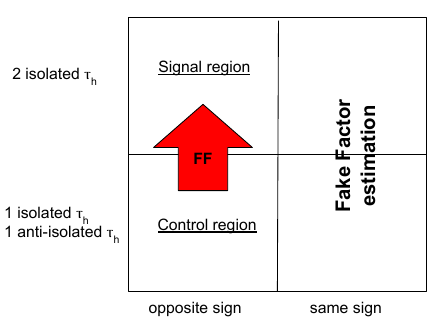
\includegraphics[width=\textwidth]{Images/FF_method.png}
  \caption{\label{fig:FF_method}}
\end{subfigure}%
\begin{subfigure}[b]{0.5\textwidth}
  \centering
  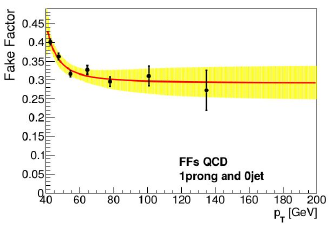
\includegraphics[width=\textwidth]{Images/FF_values.png}
  \caption{\label{fig:FF_values}}
\end{subfigure}
\caption{Illustration of the fake factor method. Diagram \subref{fig:FF_method} illustrate the way fake factors are measured, while \subref{fig:FF_values} illustrate some the values and fitted function used in the case of \tauh decaying to 1 prong and 0 jet in the event.}
\label{fig:FF_illustration}
\end{figure}

The fake factor method (FF) is used to predict all background sources where at least one of the reconstructed \tauh is actually a misidentified gluon- or quark-initiated jet. The contribution of such cases is estimated in the well-isolated signal region, defined by the presence of two offline \tauh passing all the identification criteria described in chapter \ref{sec:RECNNchapter} including the tight WP of the BDT-based isolation criterion as well the kinematic cuts of $\pt > 40\,\mathrm{GeV}$ and $|\eta| < 2.1$. This contribution is estimated from collision events in the anti-isolated signal region. The anti isolated signal region is defined by recorded events where one of the \tauh is loosely isolated but not as isolated as the signal region, which means the considered \tauh passes the loose working point of the \tauh identification criteria but not the tight. As illustrated in \ref{fig:FF_illustration}, a weight, called fake factor, is then applied to each event of the anti-isolated region to estimate the fake jet contribution in the signal region.

\begin{figure}
    \centering
    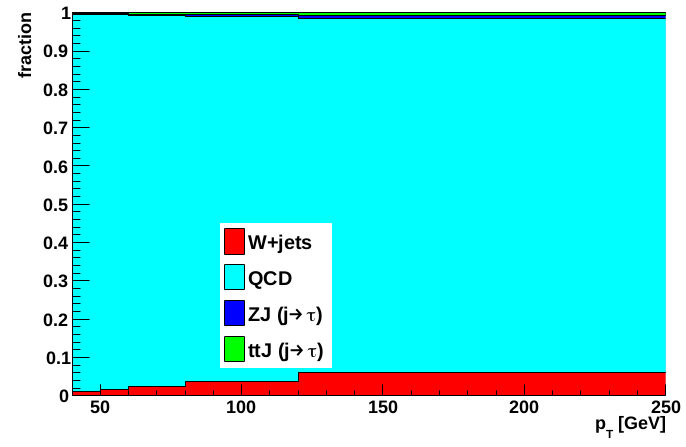
\includegraphics[width=0.45\textwidth]{Images/FF_fraction_1prong.png}
    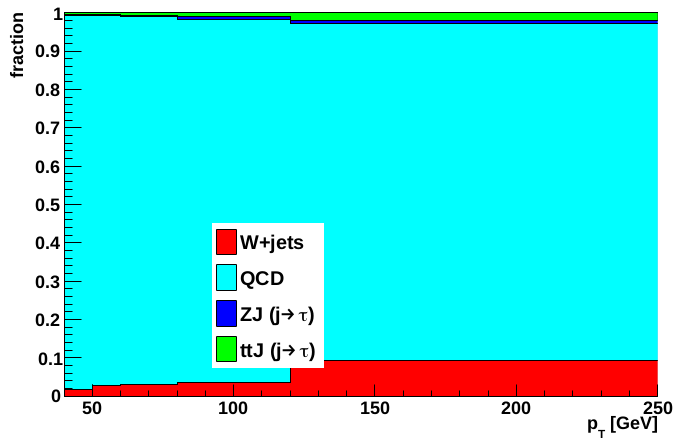
\includegraphics[width=0.45\textwidth]{Images/FF_fraction_3prong.png}
    \caption{The fractions of events from different processes in the anti-isolated signal region for 1-prong candidates (left) and 3-prong candidates (right).}
    \label{fig:FF_fractions}
\end{figure}

For all channels involving a \tauh, the fake factors are measured in different regions for each considered background process, namely QCD multi-jet, W+jets and $t\Bar{t}$. Each region is selected for their purity in the considered background. The fake factor applied to a given event in the anti-isolated region is a weighted average of the values measured for the different processes. The weight is given by the expected fraction of events of a given process in the anti-isolated region, and is binned in $m_{\mathrm{vis}}$ and number of jets. For the $\tauh\tauh$ channel, the contribution of each background is measured, as illustrated in Figure \ref{fig:FF_fractions}. Since QCD jets are the overwhelming contribution, the fake factors derived in the QCD control region are also used to estimate any other backgrounds, contrarily to the semi-leptonic channels.

In the $\tauh\tauh$ channel, the QCD fake factor measurement region correspond to events where the two reconstructed \tauh have the same electric charge sign. The value of the fake factor (FF) is then measured in this region as
\begin{equation}
    FF = \frac{\text{number of \tauh passing tight \tauh isolation discriminant}}{\text{number of \tauh passing loose but not tight \tauh isolation discriminant}} \mend
\end{equation}
The fake factors are measured as a function of the jet multiplicity (0 or $\geq$ 1) and the \pt of the anti-isolated \tauh.These measured fake factors are then extrapolated to the opposite-sign region using a correction function. This function is derived in the region where the other \tauh is also anti-isolated.  The fake factors are then interpolated by a \pt-dependent fit.

For the $\tauh\tauh$ channel, the fake factor is applied to all events in the anti-isolated region twice, once considering a \tauh as the fake, then considering the other as a fake, while multiplying both weights by $0.5$. Since genuine \tauh events in data are also present in the anti-isolated region, the expected contribution from events with genuine \tauh is subtracted in the isolated region by applying the fake factors to simulated events with genuine \tauh in the anti-isolated region.


\section{Correction of the Monte Carlo simulation}
\label{sec:MC_corr}

In order to mitigate the differences between data and simulation, several measurements have provided corrections that are applied on the simulated samples used in the analysis. These corrections are:

\paragraph{Pileup reweighting} MC simulated samples are generated with a given instantaneous luminosity which does not match the instantaneous luminosity of the data, which is often recorded after or during the production of the MC samples. In order to better fit the recorded pileup distribution in data a pileup reweighting is applied to MC events.

\paragraph{EE noise jets removal} Due to noise in the ECAL endcaps in 2017, all jets in a pseudo-rapidity gap of $2.65 < |\eta| < 3.139$ and of less than $50 \,\mathrm{GeV}$ are removed in both data and MC. The \MET is modified accordingly.

\paragraph{\tauh triggering efficiency} Trigger scale factors are also measured using a tag-and-probe method. The tag is a \tauh that passes the ID and isolation requirements applied in the analysis and is matched to a trigger \tauh object that passes the requirements of the considered trigger pattern. The probe is any \tauh that passes the ID and isolation requirements applied in the analysis, except the tag \tauh. The efficiency $\epsilon$ of the trigger is then the ratio of the number of event where the probe is matched to a \tauh trigger object to the total number of event where a probe is found. This efficiency is then computed in both data and simulation. The scale factor is then
\begin{equation}
    SF = \frac{\epsilon(\mathrm{data})}{\epsilon(\mathrm{simulation})} \mend
\end{equation}
The scale factors for the double-\tauh trigger are measured in bins of the tau \pt, $\eta$, and $\phi$. The total scale factor in the $\tauh\tauh$ is then the product of the scale factor associated to each \tauh. The scale factors for the embedded samples use the same $\epsilon(\mathrm{data})$ measured for the simulation scale factors but use the efficiency measured for the embedded taus as denominator.

\paragraph{\tauh identification efficiency} A data/simulation scale factor is measured in $\mathrm{Z}\rightarrow\mu\tauh$ events also using a tag-and-probe approach. Events with a muon and a \tauh are selected in both data and simulation and the efficiencies are extracted from a fit to the di-lepton invariant mass in the mass window around the $\mathrm{Z}$ mass. An additional correction is applied for embedded taus to correct for biases due to higher tracking efficiencies in embedded events than data.

\paragraph{\tauh energy scale} Similarly to the previous corrections, the correction on the energy of reconstructed \tauh was measured using a tag-and-probe approach in $\mathrm{Z}\rightarrow\mu\tauh$ events. This time a profile-likelihood fit is performed on the invariant mass of the muon and \tauh pair in simulation where an energscale is applied and data. The best fitted value of the energy scale for each decay mode then gives an energy correction factor that is applied to any simulated \tauh of the given decay mode.


\paragraph{Efficiency of leptons misreconstructed as \tauh} Electrons(muons) can be misreconstructed as \tauh decay products, as their track can be misinterpreted as arising from the presence of a charged hadron. As described in chapter \ref{sec:RECNNchapter}, anti-lepton discriminants are applied. A scale factor is applied to correct for the data/simulation discrepancies coming from its use. To measure these scale factors, a tag-and-probe approach is used on $Z\rightarrow e^{+}e^{-}$ and $Z\rightarrow \mu^{+}\mu^{-}$ events. The tag is then a well-identified and isolated electron(muon) and the probe is a well-identified \tauh. The efficiency is the number of \tauh probes passing the anti-lepton discriminant over the number of all found \tauh probes. The scale factor is then derived from a profile-likelihood fit performed on the visible mass distributions of events where probes that pass the anti-electron(muon) discriminant and events where the probes fail.


\paragraph{Energy scale of lepton misreconstructed as \tauh} A correction to the values of the \tauh energies for \tauh candidates originating from electron(muon) is applied for the 1-prong and 1-prong+1-\pizero decay modes \cite{Chatrchyan2011}. This correction is derived with the same approach as for the measurements of the efficiency of leptons misreconstructed as \tauh.

\paragraph{Jet energy} On top of the corrections detailed in section \ref{sec:jet_clustering}, corrections derived by the CMS collaborations to mitigate data/MC discrepancies are also applied. All the correction measurements are detailed in Ref. \cite{collaboration_2011}.


\paragraph{b-tagging efficiency} The efficiency for the tagging of b jets and the mistagging rate for light-flavour jets has been measured in both data and simulation. The efficiency and mistagging rate of the simulation is corrected through the application of efficiency and mistagging scale factors. The values of these factors and a description of the methods used to determine them can be found in Ref. \cite{Sirunyan_2018}. The simulation is corrected by un-tagging a fraction of jets that pass the requirements of b-tagging, and tagging a fraction of jets that do not pass the b-tagging requirements. The tagging of a jet is called promotion, and the untagging of a jet is called demotion. The promotion or demotion probabilities for each jet are defined as
\begin{equation*}
    P(\mathrm{demote}) = 1 - SF \msep \text{when } SF < 1
\end{equation*}
\begin{equation*}
    P(\mathrm{promote}) = \frac{(SF-1)}{\frac{1}{\epsilon}-1} \msep \text{when } SF > 1 \mend
\end{equation*}
In this expression, the scale factor $SF$ is a $\pt$, $\eta$ and jet-flavour dependant. This scale factor is the ratio of data over simulation efficiencies, and its measurement is provided by the CMS collaboration. The tagging efficiency $\epsilon$ is determined in the simulated samples used in the analysis.


\paragraph{Recoil corrections} Recoil corrections are applied to correct for the mismodeling of \MET in the simulated Drell-Yan, W+Jets and Higgs production. The corrections are derived in $\mathrm{Z}\rightarrow \mu\mu$ events, where the leptonic recoil does not contain neutrinos and the four-vector of the Z boson can be measured precisely. The effect of the recoil corrections on the \MET distribution of $\mathrm{Z}\rightarrow \mu\mu$ events, as measured by another CMS institute, is shown in figure \ref{fig:recoilcorr}.

\begin{figure}
\centering
\begin{subfigure}[b]{0.5\textwidth}
  \centering
  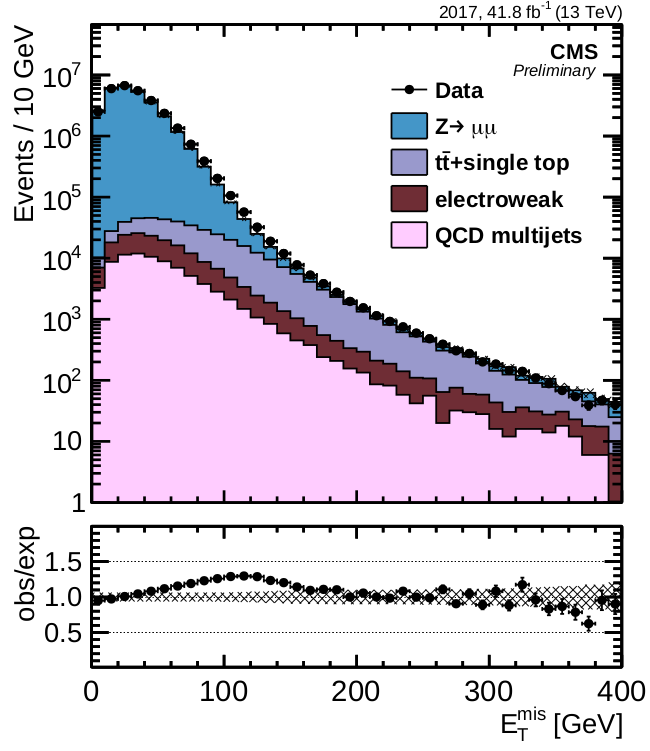
\includegraphics[width=\textwidth]{Images/withoutrecoil.png}
  \caption{\label{fig:recoil1} Without recoil corrections}
\end{subfigure}%
\begin{subfigure}[b]{0.5\textwidth}
  \centering
  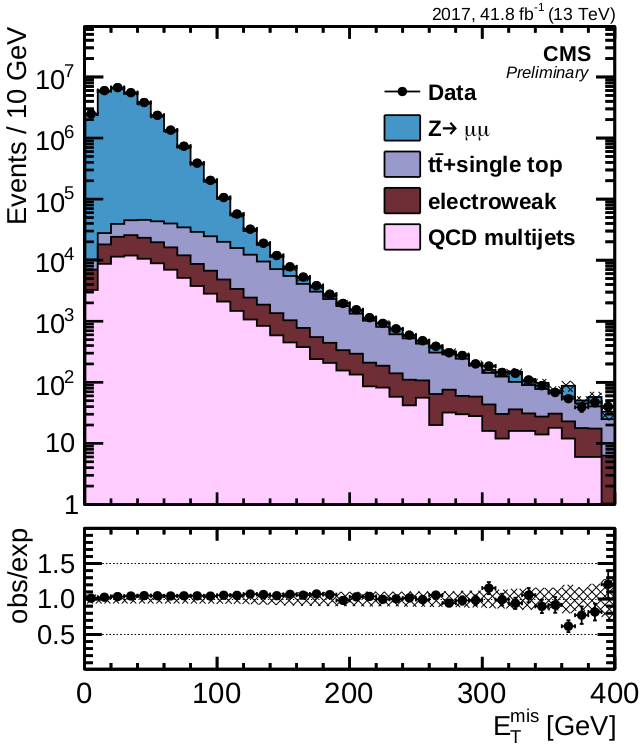
\includegraphics[width=\textwidth]{Images/withrecoil.png}
  \caption{\label{fig:recoil2} With recoil corrections}
\end{subfigure}
\caption{Effect of applying recoil corrections to the \MET distribution in the $\mathrm{Z}\rightarrow \mu\mu$ selection.}
\label{fig:recoilcorr}
\end{figure}

\paragraph{DY mass and transverse momentum reweighting} A reweighting is applied to Drell-Yan MC samples to correct the gen level di-lepton \pt and mass distributions in LO madgraph samples. These correction are measured in a $\mathrm{Z}\rightarrow \mu\mu$ control region. The weights are computed in such a way as to make the two-dimensional distributions of the $\mathrm{Z}$ \pt and the Z boson reconstructed mass match between data and simulation. The weights are then corrected not to introduce a general yield variation of the Drell-Yan background, but to only have a shape effect on the considered distributions. This correction was derived by the DESY group, and the \MET distributions of the $\mathrm{Z}\rightarrow \mu\mu$ events before and after reweighting are shown in figure \ref{fig:DYreweight}.

\begin{figure}
    \centering
    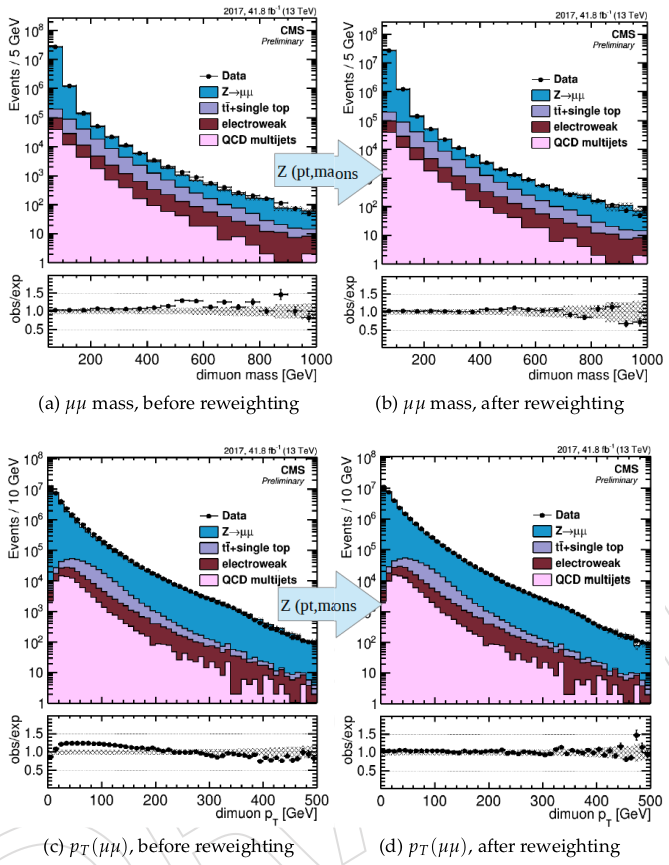
\includegraphics[width=.7\textwidth]{Images/DYreweight.png}
    \caption{Di-muon mass and \pt distributions in $\mathrm{Z}\rightarrow \mu\mu$ data before and after the DY \pt reweighting.}
    \label{fig:DYreweight}
\end{figure}

\paragraph{Top quark transverse momentum reweighting} The modeling of the $t\Bar{t}$ background is improved by reweighting the \pt spectrum of the top quarks. The correction follows the strategy developed for Run I \cite{Khachatryan:2015oqa}, as it provides the best description of this background.

% \begin{figure}
%     \centering
%     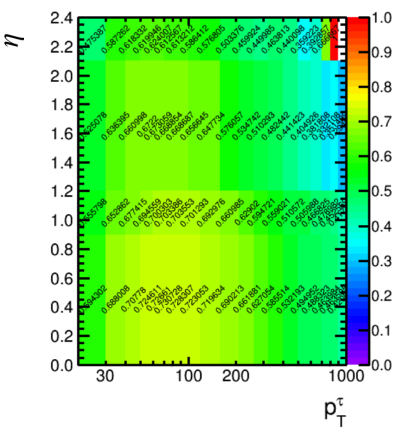
\includegraphics[width=.5\textwidth]{Images/btag_eff.png}
%     \caption{The b-tagging efficiency measured using $t\Bar{t}$ and DY MC in bins of b-jet $\eta$ and \pt.}
%     \label{fig:btageff}
% \end{figure}


\paragraph{\tauh tracking efficiency in embedded sample} In embedded events, tracking is simulated in an empty detector environment. This causes difference with respect to tracking in complete event simulation. Correction scale factors are derived by first applying the embedding technique to a simulated sample of $\mathrm{Z}\rightarrow \mu\mu$ events instead of data, and then comparing with $\mathrm{Z}\rightarrow \tauh\tauh$ simulated events.

\section{Systematic uncertainties}
\label{sec:analysis_systematics}

This section describes the sources of uncertainty that affect the signal and background predictions of the \mttot distribution in each category. The experimental uncertainties typically concern either physics object reconstruction and identification or the methods used to estimate the backgrounds described in the previous section, and are inherent to their respective measurement. The object selection is more important for the signal prediction, whereas the estimation methods have a large effect on the background estimation. Theoretical uncertainties affect the predictions of both signal and simulated background but are larger for the signal. Uncertainties can affect either the yield of the distributions only, or affect both their shape and yield. Each source of uncertainty will be represented by a nuisance parameter in the global fit described in the next section.

\subsection{Normalization uncertainties}

The yield from each process in the \mttot distribution is affected by a normalization uncertainty, described by a nuisance parameter following a log-normal distribution.

\paragraph{Luminosity} A $2.3 \%$ luminosity uncertainty is applied to the yield of contributions that are purely estimated from simulation \cite{CMS:2018elu}.

\paragraph{\tauh identification efficiency} A $7.9\%$ uncertainty is applied to the yield of contributions that are purely estimated from simulation, as well as for the embedded sample. The embedded samples also has an additional uncertainty applied to cover a tracking efficiency correction, with a magnitude of $2\%$ per \tauh.

\paragraph{Trigger efficiency} The uncertainty in the trigger efficiency amounts to $10\%$. The uncertainty is applied to all processes with a contribution predicted from simulation, and to the embedded samples. The embedded and MC uncertainties are uncorrelated. In order to account for the efficiency of the double muon trigger that was used to select input events for the embedding technique, an additional $4\%$ uncertainty ($2\%$ per muon) is applied to the embedded samples.

\paragraph{Background normalization uncertainty} A $4\%$, $5\%$, $6\%$ and $4\%$ uncertainty is applied to the $Z\rightarrow ll$, di-boson/single top, $t\Bar{t}$ and EWKZ processes, respectively, to account for the uncertainty in the production cross section of these processes. 

% \paragraph{Lepton to tau fake rate} Shape uncertainties were checked and no significant shape dependency has been observed in the event distributions used in this analysis. Therefore log normal uncertainties of $16\%$ ($26\%$) are applied for electron (muon) to tau fake rate.

\paragraph{Fake factor normalization} The uncertainty due to the subtraction of the genuine tau contribution is estimated by varying the substracted number of events by $\pm 10\%$, and amounts to about $2\%$ of the jet faking \tauh yield. %The fake factor shape uncertainties are normalized to the same area as the nominal shape, and the normalization factors are added in quadrature and act as separate nuisance parameters: this is done separately for the statistical uncertainties in the raw fake factors (about $5\%$) and the systematic uncertainties in the corrections (about $7\%$). Uncertainties are split in shape(-only) and yield uncertainties to capture the main variations induced by the uncertainties. This describes the two leading degrees of freedom of the fake factor \pt fits evaluated by toy experiments.


\subsection{Shape uncertainties}

Uncertainties that have an influence on the shape of the \mttot distribution are treated as shape uncertainties. In this case, the yield is described by a nuisance parameter following a log-normal distribution, as is done for the normalization uncertainties. The shape variations are taken into account by vertical interpolation between the \mttot histograms corresponding to a $\pm 1 \sigma$ variation, also called up or down variation respectively, of the considered source of uncertainty. The histograms corresponding to the variation of most of the uncertainties are evaluated by re-running the concerned simulated events through the analysis sequence, while applying the up or down fluctuation on the considered variable. This leads to a multiplication of the overall computing needed to perform the full analysis, and is the main reason the semi-leptonic channels are not included in this analysis yet. The following uncertainties are the ones that cause variations in the \mttot distributions.

\paragraph{\tauh Energy scale} Since the \mttot variable depends on the \pt of the selected \tauh, a separate shape uncertainty is applied for each of the corrected decay modes in the simulated samples. In the embedded samples we have hybrid events where the simulated taus might be mixed with calorimeter deposits remaining from the removal of the original muons in the events. For this reason, the tau energy scale uncertainties for embedded samples are split into two parts, where $50\%$ are fully correlated with the uncertainty for fully simulated samples and $50\%$ are uncorrelated.


\paragraph{Energy scale of leptons misreconstructed as \tauh} For the same reason, shape uncertainties are propagated to \mttot from the \pt of a misidentified \tauh arising from the presence of leptons in simulation samples uncorrelated between decay modes.


\paragraph{Jet energy} Since the change in jet energy is propagated to the \MET, the jet energy scale impacts the shape of the \mttot distribution. In general, the CMS collaboration derives uncertainties in the jet energy scale from 28 sources and combines them in a single uncertainty with one nuisance parameter. The uncertainty is split into 5 groups, instead of all 28 sources, because this would result in an unnecessary amount of parameters in the fit as well as a large technical effort. Instead, the sources are grouped according to the affected detector regions.

\paragraph{\MET unclustered energy uncertainty} The \MET takes into account the energy that is not clustered in the reconstruction process, directly impacting the value of \mttot. An uncertainty is therefore applied to all simulated processes that do not have recoil correction applied.

\paragraph{\MET recoil correction uncertainties} For all simulated processes where recoil correction are applied, uncertainties determined during the computation of the recoil corrections are propagated to the \mtot variable.

\paragraph{Top \pt reweighting} The uncertainty in the top \pt reweighting are estimated by not applying the correction (down fluctuation) and applying twice the correction (up fluctuation) in the $t\Bar{t}$ simulated events.

\paragraph{DY \pt reweighting} The uncertainty in the DY \pt reweigthing are estimated by shifting by $10\%$ the reweighting applied to $\mathrm{Z}\rightarrow ll$ events.

\paragraph{B-tagging efficiency} Categories are defined from the presence or absence of b-tagged jets in the events, therefore variation in the b-tagging of jet can lead to migration of events from one category to the other. The uncertainties in the b-tagging scale factors provided by the CMS collaboration are therefore propagated to the the \mttot distribution in the categories defined by the presence or absence of b-tagged jets.

\paragraph{\tauh tracking efficiency for the embedded samples} Since the scale factors for tracking efficiencies are dependent on the \tauh \pt, variations in their values can cause a shape effect on the \mttot distributions. An uncertainty in the tracking efficiency of hadronic taus in the embedded samples is propagated uncorrelated between 1 and 3 prong decay modes.

\paragraph{Fake-factor uncertainties} The fake factors depend on the \pt of the \tauh, and therefore a variation in those fake factor can lead to variation in the shape of the \mttot distribution. Uncertainties in the fake factor background estimation method consist of several sources:
\begin{itemize}
    \item Statistical uncertainty in the fake factor measurement in the control regions.
    \item Systematic uncertainties related to the QCD multi-jet fake factor corrections are propagated.
    \item Systematic uncertainties in the fraction of W/Z+jets events and $t\Bar{t}$ events with one misidentified \tauh in the anti-isolated region, adding two nuisance parameters. these is evaluated by varying the fractions of these two background within uncertainties (including cross section and experimental uncertainties), while readjusting the fractions of the other processes to keep the sum at $100\%$.
\end{itemize}

\paragraph{Bin-by-bin uncertainties} To account for statistical shape uncertainties in the backgrounds due to the use of Monte-Carlo and embedded samples or templates derived from data events with limited number of events, we introduce shape variations to the background templates in all categories following the Barlow-Beeston approach, where the statistical uncertainties in each bin are used to define alternative shapes.

\section{Validation}

\subsection{Fake factor method validation}

In the fully hadronic channel, the dominating contribution comes from QCD processes. Since in these processes there is no constraints between the charge of the hadronic taus, the same sign region, defined by both reconstructed hadronic taus being of the same electric charge, can be used to validate the agreement between data and the estimation method. While there is a very small correction applied to the fake factors to account for the differences between the same-sign region (SS) and  opposite-sign region (OS), the same sign distributions shown in Fig \ref{} show a good agreement between our estimation and recorded data in the SS region.

-SS region plot here

\subsection{Signal-insensitive distributions}

In order to validate our estimation methods, distributions of variables that are not sensitive to the presence of signal have been produced and the most relevant are shown in Fig. \ref{}. Other distributions can be found in appendix \ref{}.

% \subsection{Blinded distribution}

% Finally, while the \mttot distribution are used to derive conclusions on the presence of our signal, the whole range is not sensitive. Indeed, at small \mttot values, 

\section{Statistical interpretation}
\label{sec:analysis_statistical_interpretation}

This section outlines the statistical procedure used to quantify or reject the presence of a signal in data. These methods were developed by the LHC Higgs Combination Group to provide a common strategy for both the CMS and ATLAS Collaborations and to facilitate the combination of individual search results \cite{CMS-NOTE-2011-005}. 

The expected Higgs boson event yield in a given model can be denoted as $s$ and the background yield as $b$. This can refer equally to a simple counting experiment, or to predicted binned distributions for use in a shape-based analysis. An additional factor $\mu$ is introduced as a signal strength modifier, which allows for the signal rate to scale as $\mu \times s$. The background-only hypothesis is therefore defined by $\mu = 0$, and any signal hypothesis by $\mu > 0$. The term "data" will refer to an observed event count or counts, which could originate from an actual experiment or from simulation. The yields $s$ and $b$ are, in general, functions of nuisance parameters $\theta$ representing experimental and theoretical uncertainties. The nominal values $\Tilde{\theta}$ of these nuisance parameters are usually determined by external measurements, with uncertainties described by probability density functions $p(\Tilde{\theta} | \theta)$. From these components the likelihood for an observed dataset, $\Lagr(\mathrm{data}|\mu,\theta)$, is defined as
\begin{equation}
    \Lagr(\mathrm{data}|\mu,\theta) = \mathrm{Poisson}(\mathrm{data}|\mu\times s(\theta) + b(\theta)) \times p(\Tilde{\theta}|\theta) \msep
\end{equation}
where for a binned likelihood model the Poisson term is simply the product of Poisson probabilities over each bin $i$:
\begin{equation}
    \mathrm{Poisson}(\mathrm{data}|\mu\times s(\theta) + b(\theta)) = \prod_{i} \frac{(\mu s_i + b_i)^{n_i}}{n_i !} e^{-(\mu s_i +b_i)} \mend
\end{equation}

A ratio of likelihoods can be used to define a test statistic, a single number which can distinguish between two hypotheses. Such a test statistic can be used to set upper limits on the rate of signal production. Historically, a number of definitions have been used in Higgs boson searches. The one chosen by the LHC experiments is known as the profile likelihood ratio
\begin{equation}
    q_{\mu} = -2 \mathrm{ln}\frac{\Lagr(\mathrm{data}| \mu, \Hat{\theta}_{\mu})}{\Lagr(\mathrm{data}|\Hat{\mu},\Hat{\theta})} \text{, with the constraint } 0\leq \Hat{\mu}\leq \mu \mend
\end{equation}
In this expression, $\Hat{\theta}_{\mu}$ are the values of the nuisance parameters that maximise the likelihood, given the fixed signal strength $\mu$; and $\Hat{\mu}$ and $\Hat{\theta}$ are the values which give the global maximum of the likelihood. The constraint $0\leq\Hat{\mu}$ is added to prevent an unphysical negative signal strength. The constraint $\Hat{\mu}\leq\mu$ is chosen to prevent the exclusion of any $\mu$ lower than the best fit $\Hat{\mu}$, thus ensuring the construction of a one-sided confidence interval. Large values of $q_{\mu}$ indicate a value of $\mu$ that the data disagrees with, whereas values close to zero indicate good compatibility with the signal hypothesis in question. The probability of finding a value $q_{\mu}$ at least as large as the observed value, $q_{\mu}^{\mathrm{obs}}$, is defined as
\begin{equation}
    \label{eq:cl}
    \mathrm{CL}_{s+b} = \int^{inf}_{q_{\mu}^{\mathrm{obs}}} f(q_{\mu}|\mu,\Hat{\theta}_{\mu})dq_{\mu} \msep
\end{equation}
where $f(q_{\mu}|\mu,\Hat{\theta}_{\mu})$ is the probability distribution function for $q_{\mu}$. The tested value of $\mu$ is then said to be excluded at a confidence level $\alpha$, where $\alpha = 1 - \mathrm{CL}_{s+b}$. The $95\%$ CL is typically chosen when setting upper limits. One issue with this definition is that in some cases it will lead to the exclusion of low signal strengths, where an analysis has a low sensitivity. For example, this may happen with a downward fluctuation of the data when the signal expectation is very small compared to the background expectation. To protect against this effect, an additional probability $\mathrm{CL}_b$ can be introduced, defined similarly to equation \ref{eq:cl}, but under the assumption of the background-only hypothesis, $f(q_{\mu}|0,\Hat{\theta}_0)$. Instead, the ratio of these probabilities, denoted $\mathrm{CL}_s$, where
\begin{equation}
    \mathrm{CL}_s = \frac{\mathrm{CL}_{s+b}}{\mathrm{CL}_b}\msep
\end{equation}
is used to set the $95\%$ CL exclusion limit, and this is commonly referred to as the modified frequentist approach \cite{Read_2002}.

The distributions $f(q_{\mu}|\mu,\Hat{\theta}_{\mu})$ and $f(q_{\mu}|0,\Hat{\theta}_0)$ can be determined by generating toy MC datasets from their respective models, in which the nuisance parameters are fixed to the values found in the fits to the observed data. The value of $q_{\mu}$ is then determined for each toy dataset. The effect of systematic uncertainties is incorporated by sampling a set of pseudo-measurements $\Tilde{\theta}$ in each toy using the chosen nuisance pdfs. It is often instructive to compare the observed exclusion limit to the expectation under the assumption of the background-only hypothesis. This can be determined by generating background-only toy datasets and determining the $95\%$ CL limit in each. These values form a cumulative pdf from which the median exclusion and uncertainty bands can be extracted.

A profile likelihood ratio can also be used to calculate the p-value for an observed excess of events given the background-only hypothesis. For this a slightly modified definition of the test statistic is required,
\begin{equation}
    q_0 = -2 \mathrm{ln}\frac{\Lagr(data|0, \Hat{\theta}_0)}{\Lagr(data|\Hat{\mu}, \Hat{\theta})}, \text{ with the constraint }\Hat{\mu} \geq 0\msep 
\end{equation}
where the constraint $\Hat{\mu} \geq 0$ is chosen to prevent a downward fluctuation being considered evidence against the background-only hypothesis. The p-value for the observed data is then given as
\begin{equation}
    p_0 = \lim^{\inf}_{q_o^{\mathrm{obs}}} f(q_0 | 0, \Hat{\theta}_0) dq_0\msep
\end{equation}
where $f(q_0 | 0, \Hat{\theta}_0)$ can be determined by generating pseudo-data from the background-only hypothesis. The p-value is typically converted to a significance, Z, by determining the number of standard deviations of a one-sided normal distribution that would yield an equal tail probability.

A major advantage of the profile likelihood test statistic is that in the limit of a large data sample, the distribution $f(q_{\mu})$ follows a known formula \cite{Carena2013}. This so-called asymptotic limit approximation removes the need for the computationally intensive step of generating and fitting toy datasets, which can take an appreciable time for models with many bins and nuisance parameters. This method relies on the properties of the Asimov dataset, a single representative dataset in which the observed rates match exactly the prediction of the model under the nominal set of nuisance parameters. Furthermore, it is possible to derive a formula for the median expected limit and uncertainty bands using only the properties of the Asimov dataset, thus completely removing the need for any toy MC \cite{Carena2013}.

\section{Results and interpretations}
\label{sec:analysis_results}

The statistical interpretation in the MSSM includes the use of a simultaneous maximum-likelihood fit of the \mttot distribution in the two categories, namely b-tag and no b-tag categories.  Once the \mttot distributions are created, a fit under the background-only hypothesis is performed on both categories. The resulting distributions are shown in Fig. \ref{}.
-postfit (b-only) plots in both categories without signal

\begin{figure}
    \centering
    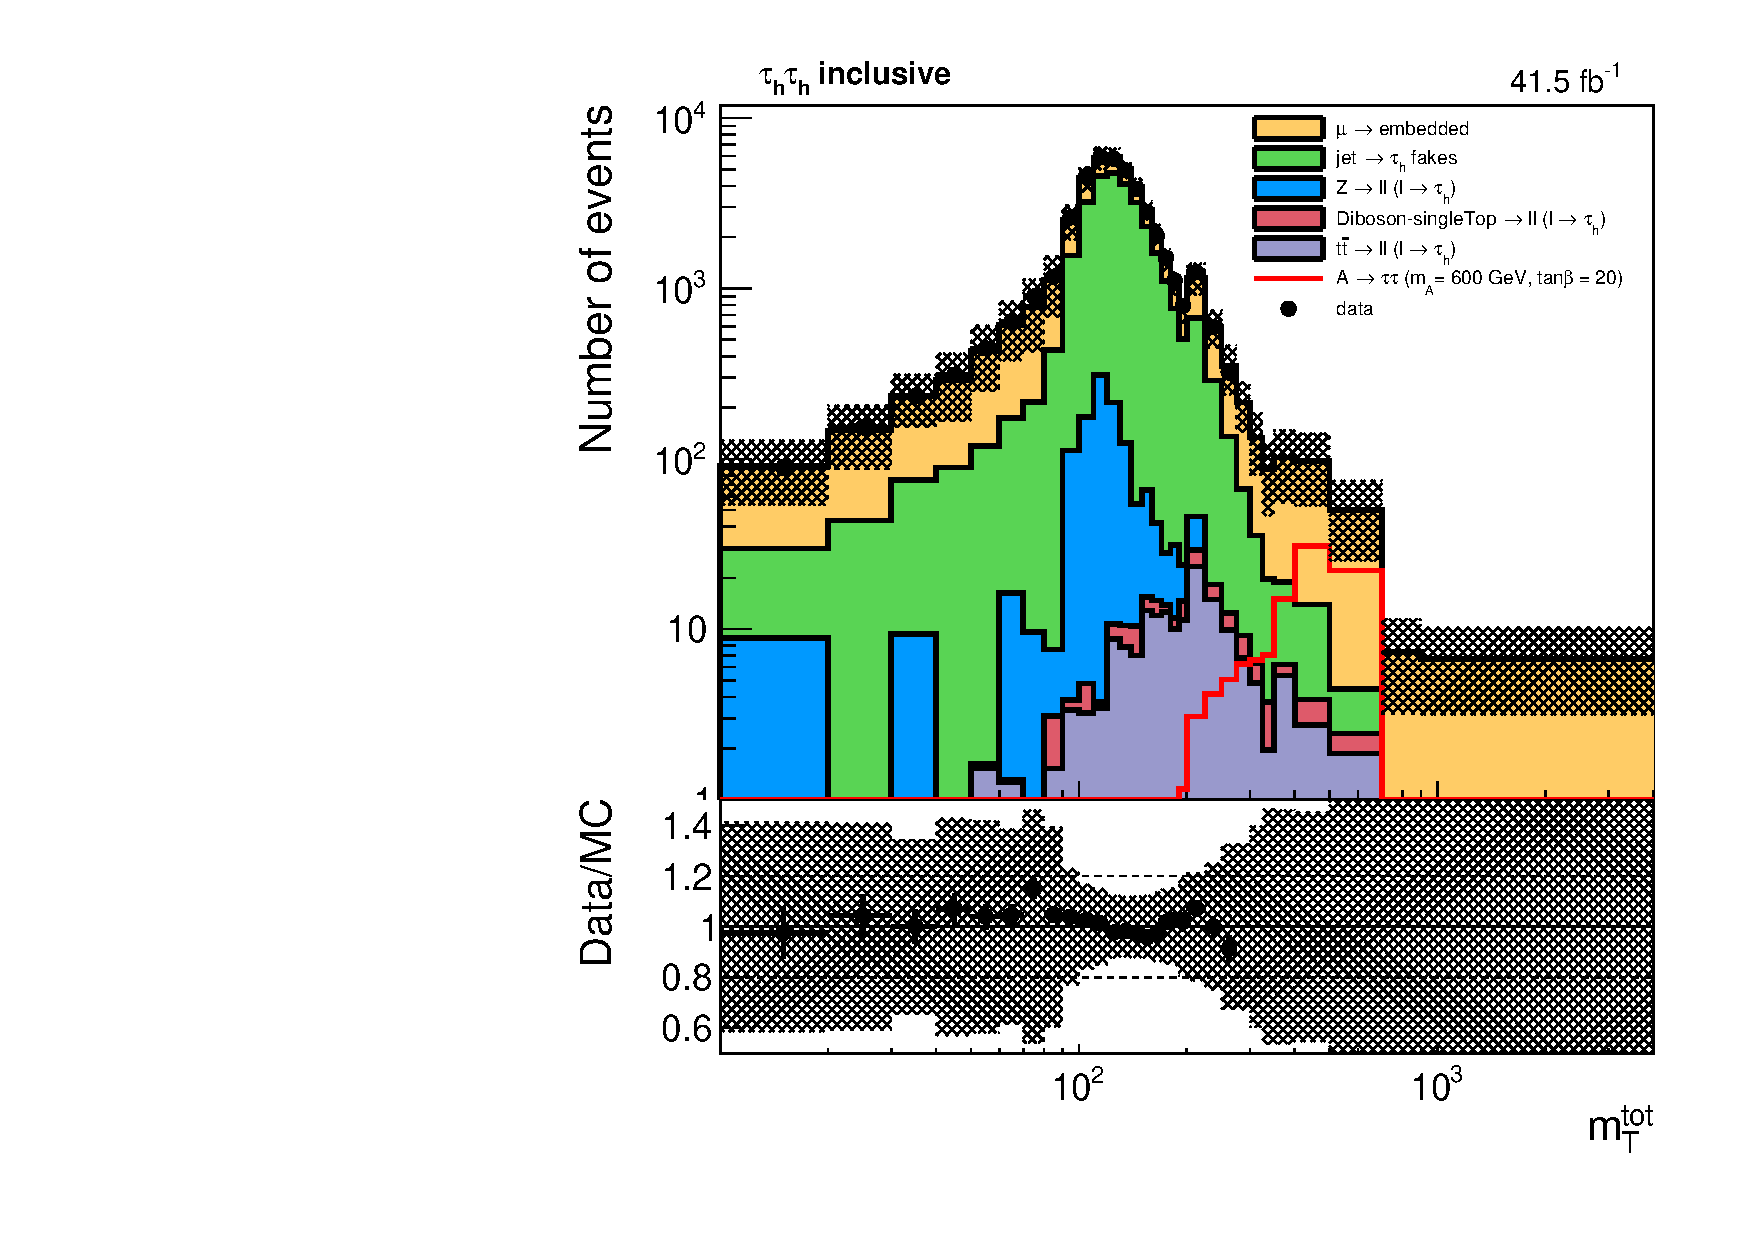
\includegraphics[width=0.45\textwidth]{Images/prefit_plots_tt_inclusive.pdf}
    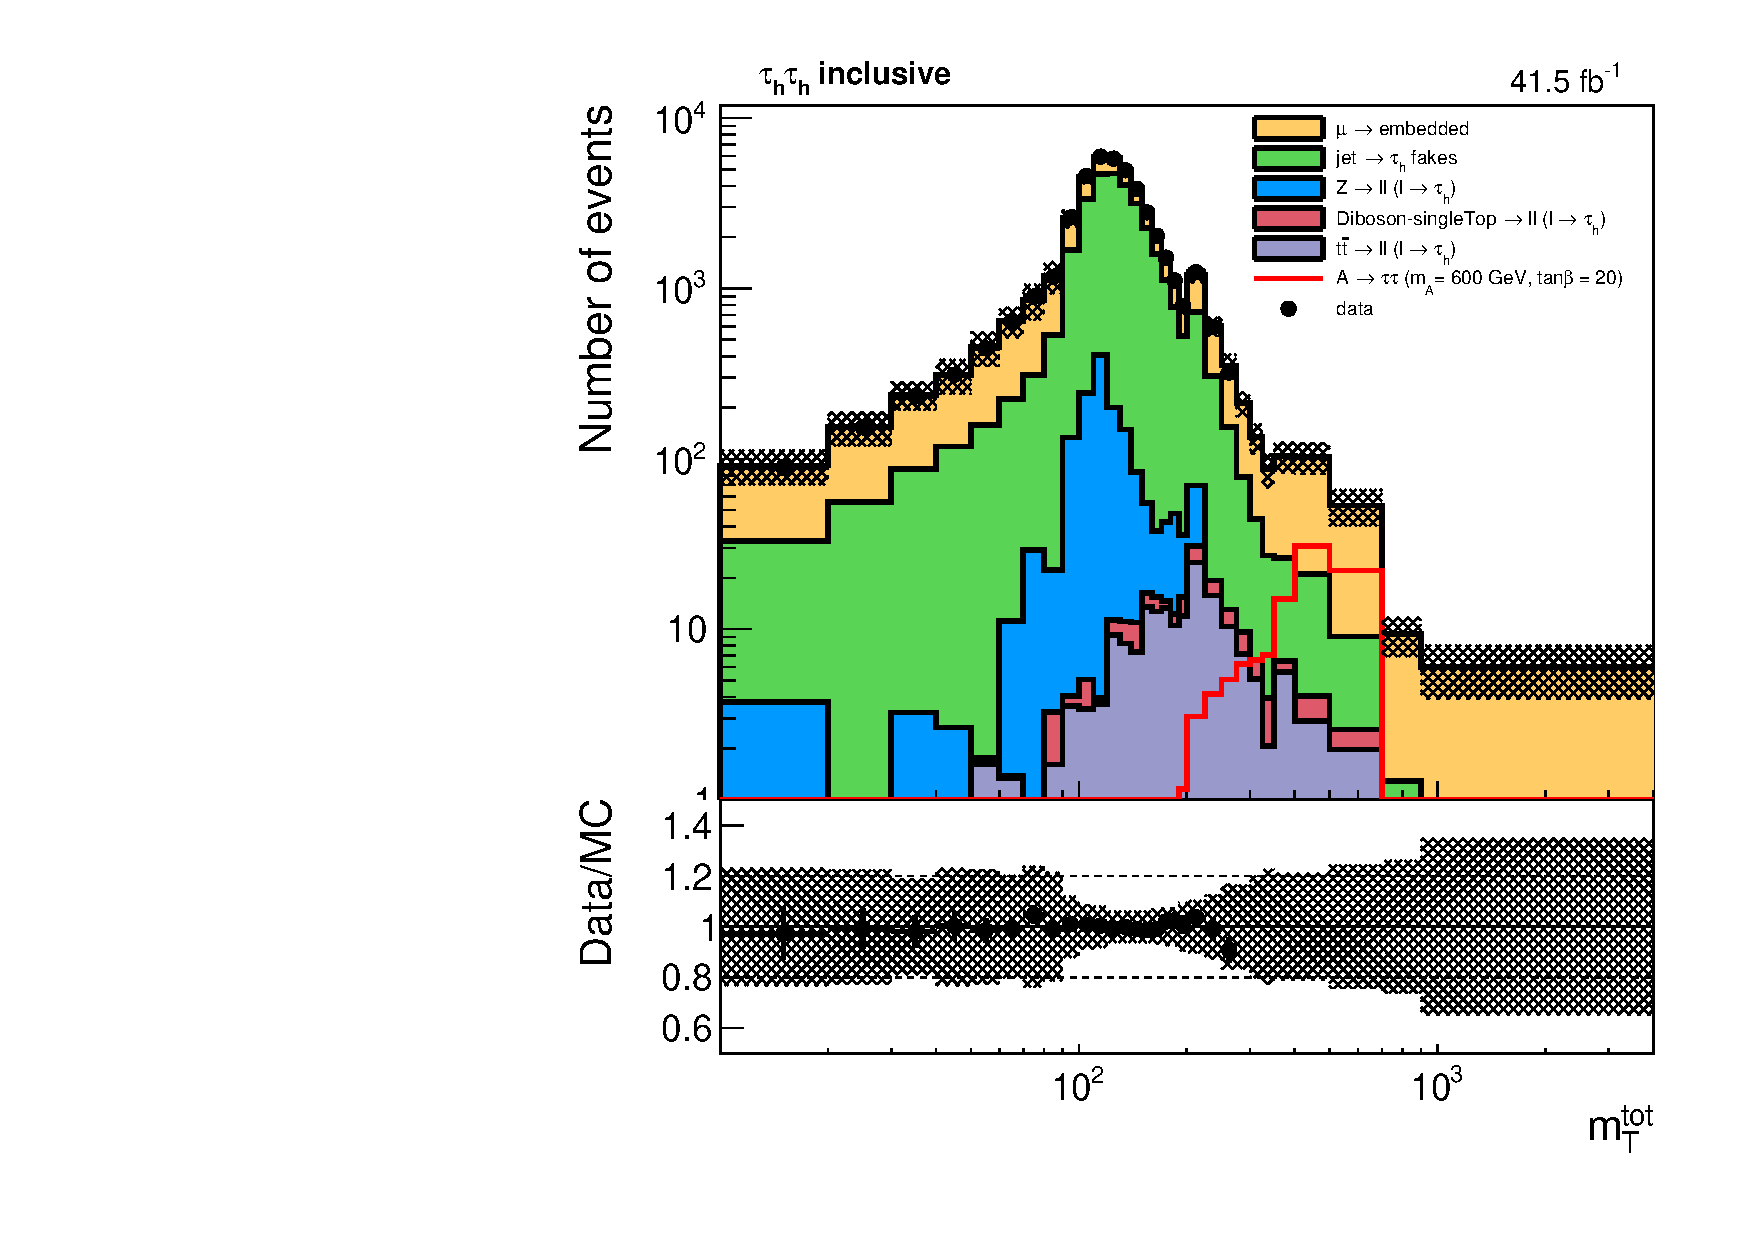
\includegraphics[width=0.45\textwidth]{Images/postfit_b_plots_tt_inclusive.pdf}
    \caption{Distribution of \mttot in the inclusive category prefit (left) and post background-only fit.}
    \label{fig:control_plots}
\end{figure}

\begin{figure}
    \centering
    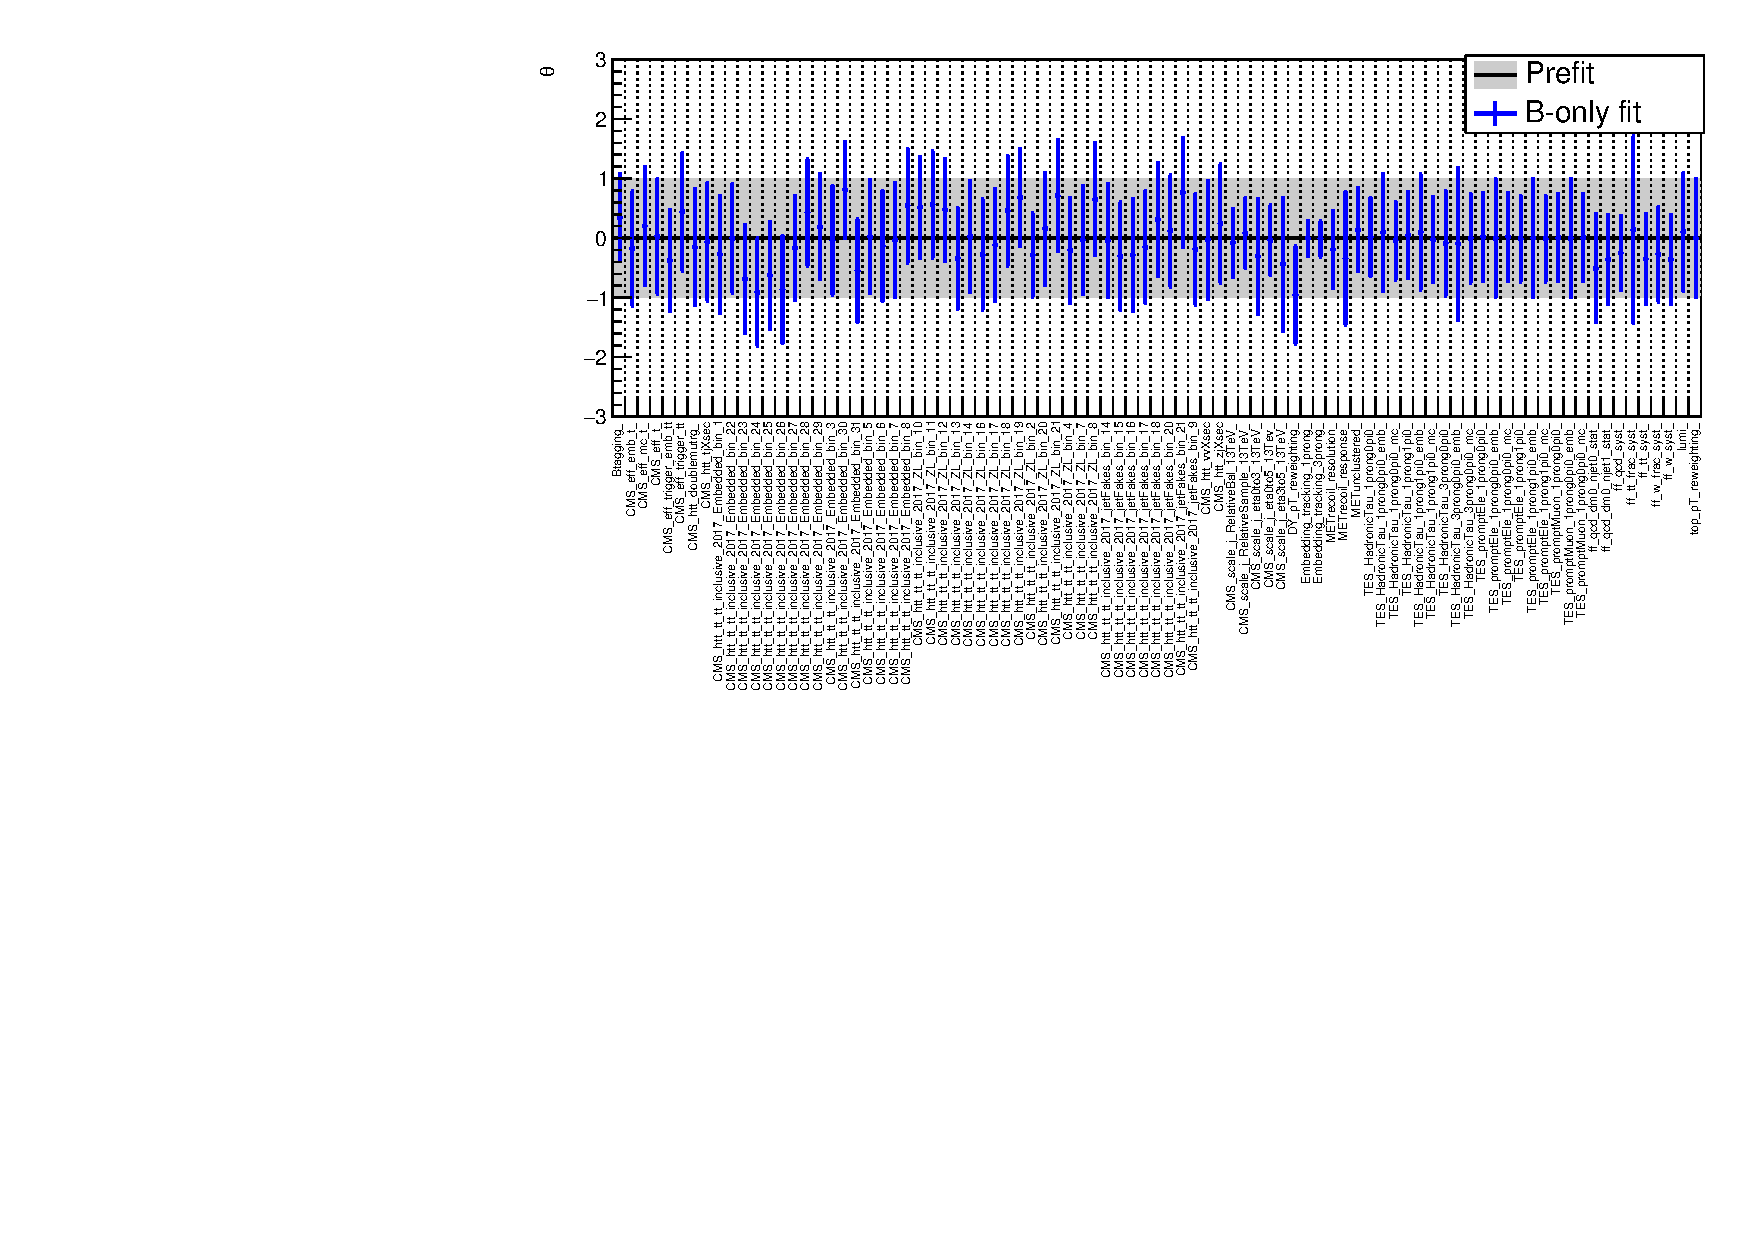
\includegraphics[width=\textwidth]{Images/nuisances.pdf}
    \caption{Values of the nuisance parameters from the background-only fit.}
    \label{fig:nuisances}
\end{figure}
% Figure \ref{fig:control_plots} give the \mttot distributions for the inclusive category, both before and after the background-only hypothesis fit. The signal expectation is given for the \mhmax scenario with \ma $= 600\,\mathrm{GeV}$ and $\mathrm{tan}\,\beta = 20$. Following the blinding procedure, the yield of data in bins sensitive to the presence of signal is hidden. The unblinding process for this data is to be started after the writing of this manuscript. Figure \ref{fig:nuisances} gives the relative change of each nuisance parameter used in the fit with respect to its nominal value. The most constrained nuisance parameter is the shape uncertainty related to the DY \pt reweighting, which only impacts the $\mathrm{Z}\rightarrow ll (l\rightarrow \tauh)$ process estimation. As all other nuisance parameters are within the statistically determined uncertainties from their nominal value, which means the fit did not have to constrain any of these sources of uncertainty outside of their estimated uncertainty. 


Upper limits in this search are determined in two different ways. The first context is for model-independent limits on the cross section of a single neutral Higgs boson, denoted $\Phi$, produced either through the gluon-gluon fusion or b-associated production mode and decaying to $\tauh\tauh$. The second is in the \mhmax scenario, where limits on the parameter  $\mathrm{tan}\,\beta$ are determined as a function of \ma. In this case, the signal model includes the three neutral Higgs bosons h, H and A with masses, cross and branching ratios computed from the chosen values of \ma and $\mathrm{tan}\,\beta$. The following paragraphs detail how those searches will be performed.


Signal samples are generated for the set of \ma mass points to be tested, in the range $90$ to $3200\,\mathrm{GeV}$. The step size between points increases with \ma to scale with the worsening \mttot resolution. To derived model-independent expected upper limits on the production of a single neutral Higgs boson with mass $m_{\Phi}$, fits under the signal plus background hypothesis will be performed. The limits on the cross section times branching fraction, $\sigma\times B(\Phi\rightarrow\tauh\tauh)$, will be determined individually for gluon-gluon fusion and b-associated production. In the fit to extract gluon-gluon fusion limits the b-associated contribution will be allowed to float freely, and vice versa. This is required as neither the no b-tag or b-tag categories are completely pure in one production mode, and this avoids the need to impose any assumptions about the ratio of cross sections between the two processes.

-In order to allow the evaluation of the limit at different mass points, including between the mass points for which simulation has been processed, a horizontal morphing \cite{READ1999357} is used. All available processed templates are used for the template morphing and the template fit is performed using the distributions produced by the morphing.

- ggh bbh limits plots

% \begin{figure}
%     \centering
%     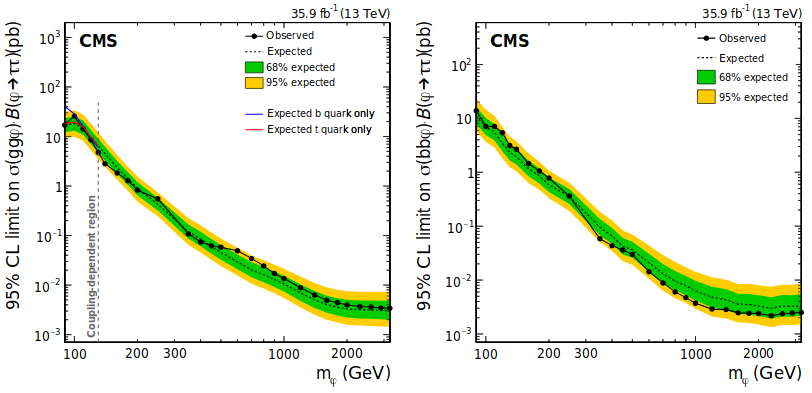
\includegraphics[width=\textwidth]{Images/xslimitsMSSM.png}
%     \caption{Expected and observed $95\%$ CL upper limits for the production of a single narrow resonance, $\Phi$, with a mass between $90\,\mathrm{GeV}$ and $3.2\,\mathrm{TeV}$ in the $\tauh\tauh$ final state (left) for the production via gluon fusion (gg$\Phi$ and (right) in association with b quark (bb$\Phi$). The expected median of the exclusion limit is shown by the dashed line. The dark green and bright yellow bands indicate the 68 and 95$\%$ confidence intervals for the variation of the expected exclusion limit. The black dots correspond to the observed limits.}
%     \label{fig:xslimits}
% \end{figure}



A number of additional steps are needed to determine the \ma -  $\mathrm{tan}\beta$ limits. At each \ma -  $\mathrm{tan}\beta$ hypothesis, the masses of the other two Higgs bosons are calculated using results from the Higgs Working Group \cite{Dittmaier:1318996}. In each event category, templates for the h and H are generated by the horizontal morphing \cite{READ1999357} between templates from the two closest samples in mass. The category acceptance is similarly interpolated from the neighbouring mass points. All three templates are scaled by the appropriate cross sections and branching ratios and combined into a single template. The $95\%$ CL upper limit is determined for each point on the \ma -  $\mathrm{tan}\beta$ grid, with the signal strength parameter $\mu$ uniformly scaling the entire signal model. The limit in  $\mathrm{tan}\beta$ is then defined as the point on which this upper limit is found to occur at $\mu = 1.0$. Practically, this is determined by interpolation between the points on either side of this threshold.

-ma-tanbeta plots

% The SM Higgs boson can be added to the background processes. This would turn the likelihood ratio into a comparison between the MSSM and the SM Higgs sector hypotheses.


% The expected limits for the MSSM $m_{\mathrm{h}}^{\mathrm{mod}+}$ and the hMSSM scenarios are given in figure \ref{fig:limits}.

% \begin{figure}
%     \centering
%     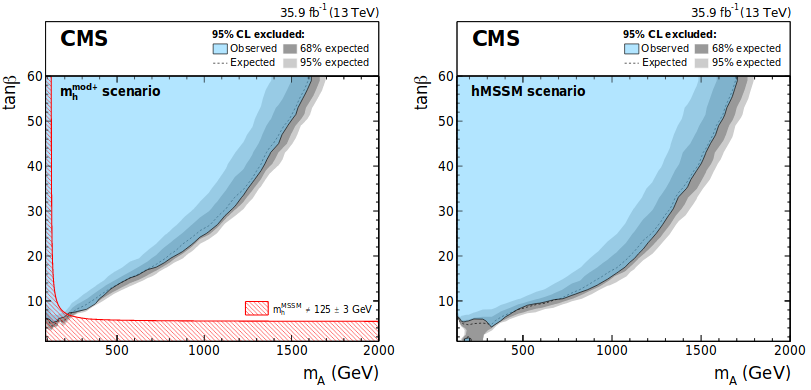
\includegraphics[width=\textwidth]{Images/MSSMlimits.png}
%     \caption{expected and observed $95\%$ CL exclusion contour (left) in the MSSM $m_{\mathrm{h}^{\mathrm{mod}+}}$ and (right) in the hMSSM scenarios. The expected median is shown as a dashed black line. The dark and bright gray bands indicate the 68 and 95 $\%$ confidence intervals for the variation of the expected exclusion. The observed exclusion contour is indicated by the coloured blue area. For the $m_{\mathrm{h}}^{\mathrm{mod}+}$ scenario, these parts of the parameter space, where $m_{\mathrm{h}}$ deviates by more than $\pm 3 \,\mathrm{GeV}$ from the mass of the observed Higgs boson at $125\,\mathrm{GeV}$ are indicated by a red hatched area.}
%     \label{fig:limits}
% \end{figure}


